\chapter{Mental Health}

% frame the chapter
Increasingly recognized as a crucial factor for well-being, mental health carries significant economic implications that are often overlooked in favor of more easily quantified conditions, such as physical health. Nevertheless, recent events such as the COVID-19 pandemic shed light on the importance of psychological welfare. 

% economic relevance (social capital, productivity)
Mental health is an economically relevant phenomenon with far-reaching implications that extend beyond individual well-being. Poor mental health often leads to reduced productivity, increased absenteeism, and higher turnover rates in the workplace, directly impacting an organization's bottom line (OECD/EU (2018), OECD/EU (2022)). Furthermore, it places a significant burden on healthcare systems through increased medical costs and utilization of services. The indirect costs, such as loss of income due to disability and the ripple effects on families and communities, further amplify its economic relevance and far outweigh the direct healthcare costs (OECD/EU (2022), WHO (2022)). Therefore, investing in mental health not only enhances individual quality of life but also has the potential for significant economic returns, framing it as a key opportunity in the context of social capital accumulation.

This chapter aims to shed light on the definitions, statistics and dynamics of the topic, with the aim of providing the reader with comprehensive and up to date knowlege in this realm. 

\section{Defining mental health}
% what is MH in general 
    Mental health can be defined as a state of psychological well-being which allows people to cope with demands of life, realize their abilities, learn and work well while contributing to their community. It represents a crucial feature of personal and collective socio-economic develpoment, involving psychological, emotional and social welfare, and affecting how people think, feel and act. 
    Being mentally healthy goes beyond the mere absence of clinically relevant conditions, it encompasses self-esteem, resilience, relationships. Conditions that affect mental health include mental disorders, psychosocial disabilities and mental states associated with impaired functioning, or risk of self-harm. Those affected by these conditions are more likely to report lower mental well-being. 

    % MH risk factors
    Mental health is dynamic and is affected by the interplay of biological factors, environmental conditions and individual experiences. Biological factors such as genetics or substance abuse can create vulnerabilities in all stages of life, but events that occur during developmentally sensitive periods are particularly impactful. Harsh childhood experiences in the form of bullying, physical or psychological abuse and poor health can have long lasting negative consequences on an individuals' mental condition. On the other hand, mental resilience can be promoted through building social and emotional skills, providing youths with positive interactions, safety and community as well as quality education. 
    Thus, mental health can be though of as a continuum ranging from an optimal state of well being, to debilitating states of great suffering and emotional pain (WHO, 2022).

    When dealing with circumstances that can exacerbate mental ill-health, a distinction can be made between local factors which affect individuals, families and communities on a small scale, and global or systemic factors which generate vulnerabilities for the entire population. Among the latter we find key threats such as economic crises, disease outbreaks, humanitarian emergencies, displacement and climate crisis related events, as well as sociocultural and geopolitical factors such as infrastructure, inequality, social stability and environmental quality. 
    
    % MH protective factors
    Although exposure to risk factors undermines mental health, most at-risk people will not develop conditions, while many without known risk factors will develop them. In this perspective, encouraging protective factors strenghtens resilience in the population. On the individual plane, building strong social and emotional skills, a solid sense of self-worth and healthy habits such as keeping physically active are key in generating resilient individuals. Other individual protective factors include a nurturing and supportive family environment from a very young age, decent working conditions and a cohesive social network. On the structural level, protective factors manifest in economic security, easy and equal access to services, social protection, qualitable infrastructure and economic security, as well as social integration and contained inequality.  


        



\section{Global epidemiological overview}
    % define relevant MH issues --> depression, anxiety, suicide stats
    Mental health conditions are prevalent in the population, with about one in eight people worldwide living with a mental disorder (WHO, 2022). Heterogeneity in their distribution emerges according to age, gender and other individual characteristics. Overall, disorders related to anxiety and depression are the most common, and suicide accounts for more than one out of one hundred deaths (WHO, 2022). 
    % seeking help
    Still, seeking help for mental health conditions is hindered by low mental health literacy, poor service quality, high cost of care, fear of stigma and discrimination, making for underdiagnosis of all conditions. 

    % service provision not commisurated with needs
    Worldwide, mental health conditions are severely underserviced due to lack of information and research, as well as deficient provision of resources and services. On average, less than 2\% of healthcare budgets are dedicated to mental health, and out of that more than 70\% of mental health expenditure in middle-income countries is dedicated to psychiatric hospitals (WHO, 2022). 
    Furthermore, professionals such as psychiatrists and psychologists are scarce relative to the population, and gaps in service coverage are amplified by quality and cost of care across countries. 
    % measurement challenges
    Additionally, measurement of mental health condition is hampered by incomplete data, outdated information and cross-cultural differences in the conceptualization and tracking of conditions.

    % quick stats
    The most commonly occurring mental conditions are anxiety disorders, which have a prevalence rate of about 4\%, followed closely by depressive disorders at 3.8\%. Developmental disorders and Attention Deficit Hyperactivity Disorder (ADHD) are also significant, contributing to an additional 1.4\% and 1.1\% of cases, respectively (WHO, 2022).
    A higher percentage of the population is diagnosed in high-income countries, followed in order by middle and low-income countries (WHO, 2022). On average, people with severe mental conditions die 10-20 years prematurely with respect to the general population (Chesney et al., 2014) and at great individual and societal cost. 
    % this section
    This section presents current statistics on the global prevalence and diversity of mental health conditions, with a particular emphasis on the OECD region prior to the COVID-19 pandemic. Before delving into a data-driven discussion on this subject, it is essential to first clearly define the two most pertinent categories of mental disorders under consideration: anxiety and depressive disorders. 


        \subsection{Anxiety disorders}

            \begin{figure}  % anxiety OECD rates figure
                \centering
                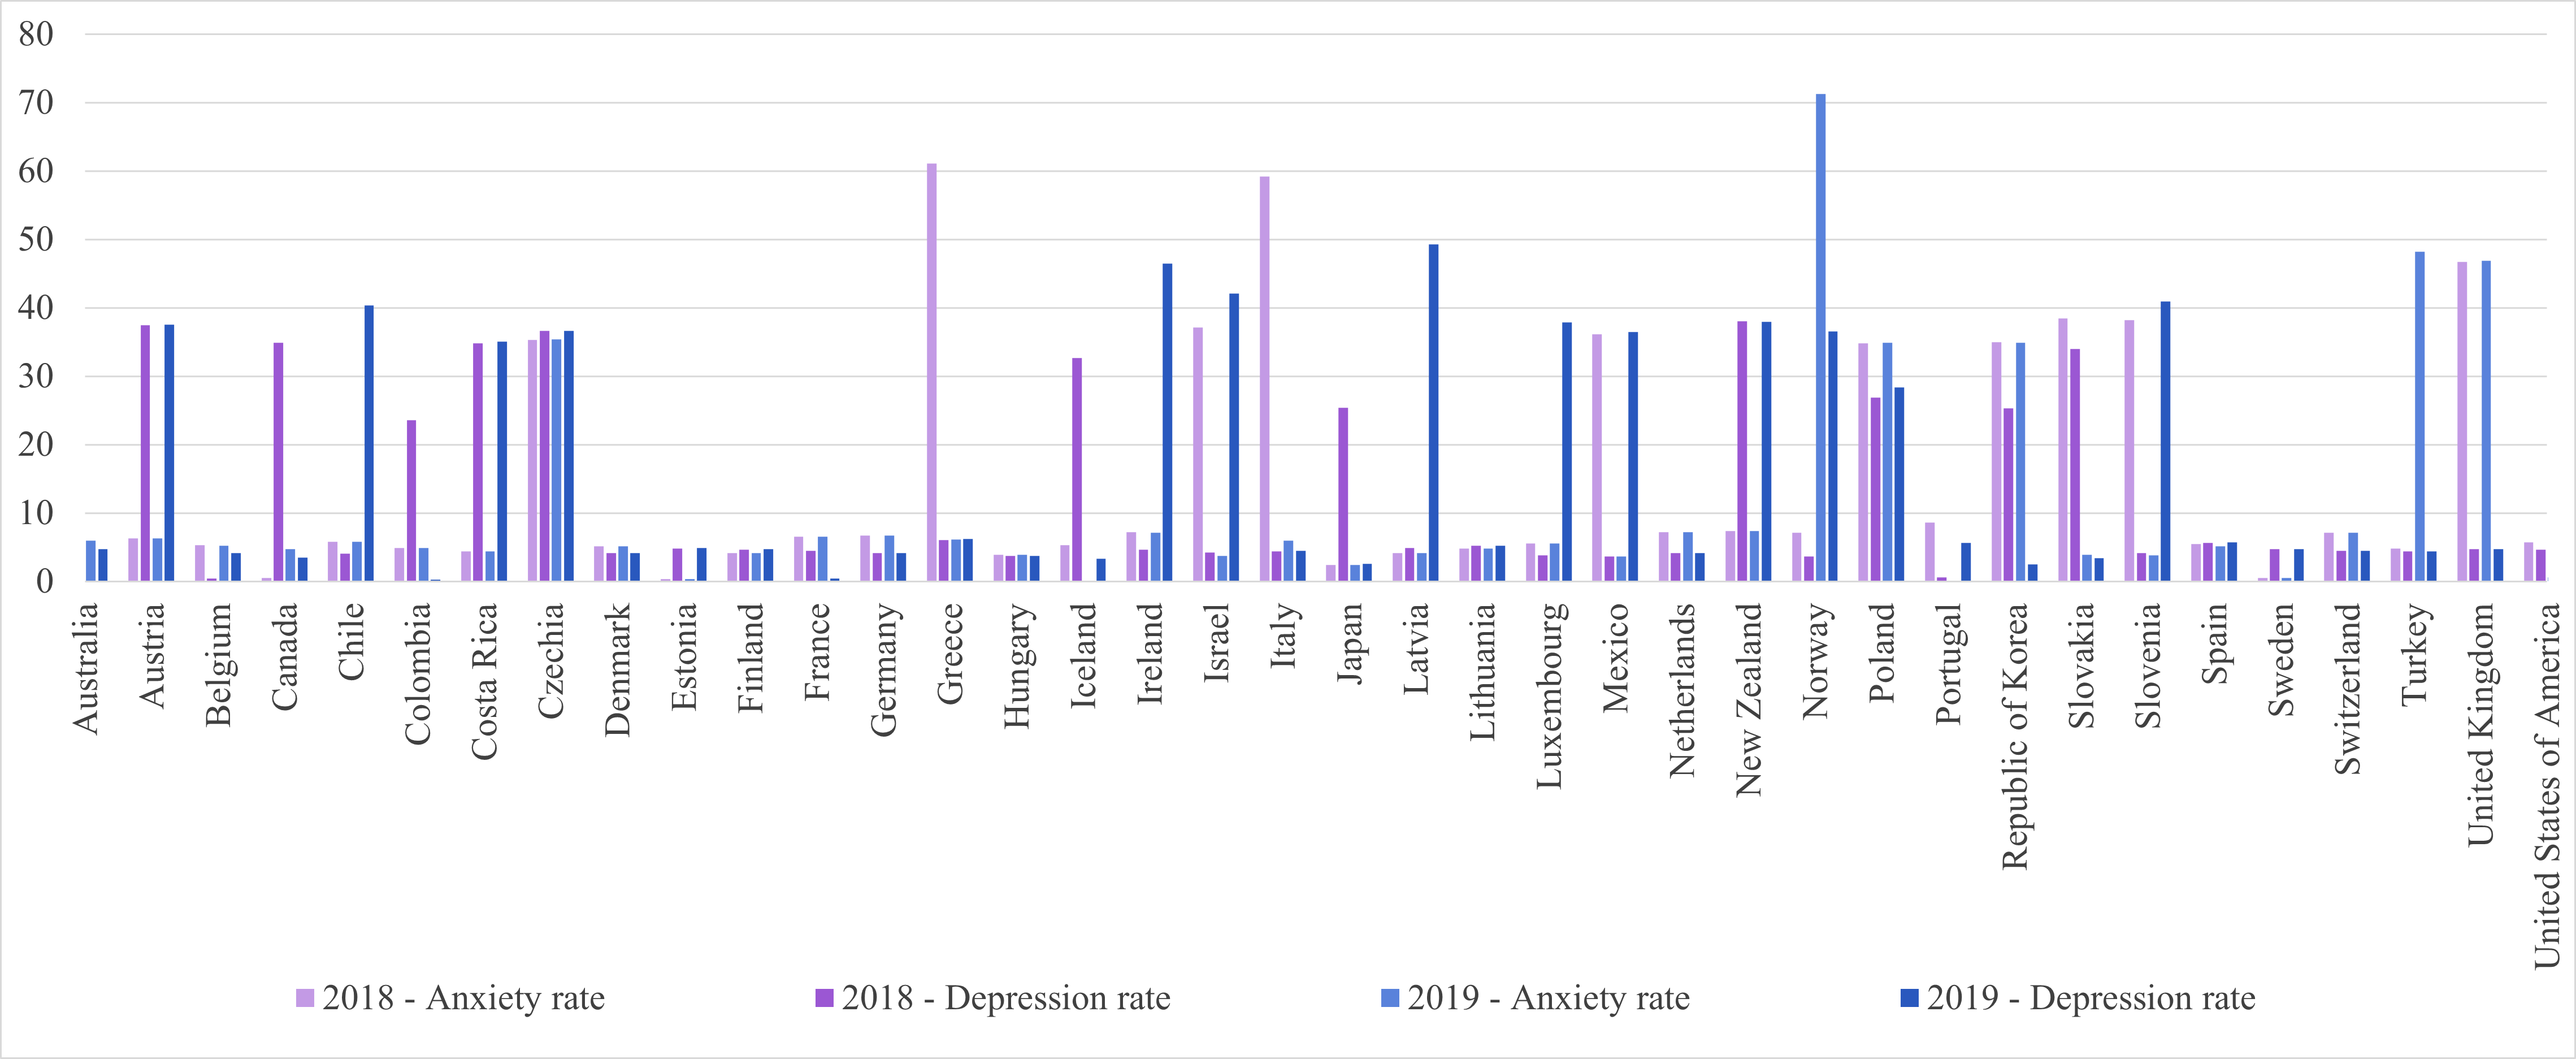
\includegraphics[width=\textwidth]{GRAPHS/anxiety_depression_100_rate_2018_2019.png}
                \caption{\emph{Prevalence of anxiety and depression disorders per $100$ inhabitants, 2018-2019.}
                {\scriptsize Source: Global Burden of Disease Study 2019 (GBD 2019), available from https://vizhub.healthdata.org/gbd-results/.}}
                \label{fig:anxiety_OECD}
            \end{figure}
            
            % DSM-V 
            Anxiety disorders involve excessive and prolonged feelings of worry, fear, or nervousness that negatively affect an individual's ability to function. According to the Fifth Edition of the Diagnostic and Statistical Manual of Mental Disorders (DSM-5), they are classified as follows: separation anxiety disorder, selective mutism, specific phobia (related to animals, natural environment, blood, injection, injuries, specific situations or other), social phobia, panic disorder, panic attacks, agoraphobia, generalized anxiety disorder (GAD). Comorbidity of anxiety disorders is most common with depression and substance abuse (DSM-5, WHO (2022)).

            The symptomatology includes physical symptoms that often include but are not limited to heart palpitations, muscle tension, and gastrointestinal discomfort. Behavioral symptoms manifest as avoidance behaviors, such as evading places or situations that trigger anxiety. On a psychological level, patients experience a heightened state of arousal and hyper-vigilance, frequently leading to intrusive thoughts and emotional distress. These symptoms are not static but interact in a dynamic fashion, often exacerbating each other in a vicious cycle that hampers the quality of life for the affected individual.


        % depression    [  %  TO DO  %  ]
        \subsection{Depressive disorders}
            According to the DSM-5 the main categories of depressive disorders are: major depressive disorder (MDD), persistent depressive disorder (dysthymia), bipolar depression, depressive disorder as a consequence of other medical conditions, and substance induced depressive disorder. For the disorder to be clinically relevant, the DSM-5 criteria must be met alongside functional impairment.
            Depressive disorders are often comorbid with anxiety disorders and substance abuse. 

            Core symptoms of this category include depressed mood, characterized by feelings of hopelessness, despair and sadness, and a significant loss of interest or pleasure in activities, also known as anhedonia. Depressive disorders are also characterized by the presence of cognitive symptoms such as reduced concentration, indecisiveness, feelings of worthlessness and guilt, and suicidal ideation. Additionally, symptoms may manifest physiologically through changes in appetite and weight, disturbed sleep, psychomotor issues in the form of agitation or retardation, and fatigue. Finally, an affected individual may show affective manifestations such as a lack of emotional responsiveness and irritability. 
        \subsection{Heterogeneity determinants of mental health conditions}
            Factors which generate heterogeneity in mental  health measurement and statistics are gender, age, socio-economic status, ethnicity, geographic location, cultural background, sexual orientation. Furthermore, different diagnostic criteria and data collection methods complicate cross-country comparison. 
            For instance, cultural background adds a layer of complexity in the case of stronger stigma towards mental illness, which makes symptoms less readily identifiable and individuals more prone to masking their conditions.  
            To further exemplify the complexity from the interplay of the aforementioned factors, the reader may consider the fact that worldwide about 4\% of people live with anxiety disorders, but this number increases to 10\% for working age women in the Americas (WHO, 2022). 
        
            In this analysis, two of the most poignant determinants of heterogeneity are gender and cohort. 


    % statistics using WHO and EUROSTAT data references
    \paragraph{Gender differences.}
        % differences in diagnosis
        Women and men often display different prevalence rates and patterns of mental health issues.
        On average, women are more likely to be diagnosed with mood and anxiety disorders, such as depression and generalized anxiety disorder, while men are more prone to be diagnosed with substance abuse and externalizing disorders like conduct disorder (WHO, 2022). Worldwide, 13.5\% of women live with a mental disorder, as opposed to 12.5\% of men (WHO, 2022). 
        % pregnancy
        Factors such as pregnancy increase the risk of all mental conditions, especially depression. Woody et al. (2017) find increase prevalence of symptoms in women from low and middle income countries in the perinatal period. 
        % symptomatology of disorders
        Alexandrino-Silva et al. (2012) analyze symptomatics subtypes of depression and their relation to gender. For the most symptomatic classes of the disorders, they find women reporting more inhibition and disturbances to sleeping and eating patterns, and hypersomnia. Men reported more psychomotor retardation and agitation. 

    % MEN MORE LIKELY TO DIE SUCIDE    [   CHECK   ]

    \paragraph{Cohort specificity.}
    % youth and old more affected
    A study by Bell (2014) challenges the belief of a U-shaped life course trajectory in mental health, using data from the British Household Panel Survey, arguing that previous literature had not properly separated age, period, and cohort effects. Key findings show that mental health does not follow  U-shaped trajectory, instead, it increases throughout life, slowing down in mid-life, and worsening again in old age. Cohort effects also play a role, with more recent cohorts showing worse mental health. 
    On average, youths and older adults suffer most from mental conditions; WHO (2022) data shows that around 8\% of children aged 5-9 and 14\% of adolescents ages 10-19 live with a mental condition. For adults 70 years and older, around 13\% live with a mental disorder (excluding dementia), mostly in the form of depressive and anxiety disorders. Within this age category, affected women are 14.2\% and men 11.7\%.

    % onset
    The analysis of a nationally representative survey in the United States done by Kessler et al. (2005) shows that the median age for onset is 11 years for anxiety disorders, 20 years for substance abuse and 30 years for mood disorders. Overall, three fourths of all lifetime conditions have onset before 24 years of age. 

    % old people problems: depression, anxiety, suicide, isolation      [   COMPLETE    ]
    In the older population, depression is associated with emotional suffering and increased suicidal ideation, and a risk factor for disability and mortality (Zenebe et al. (2021), Vieira et al., (2014)). Many of the risk factors for depression are associated with increased age, such as social isolation, traumatic life events, functional decline, loss of independence and onset of medical conditions. Depression in older adults is associated with events such as falls, strokes, functional ipairment, activity limitations (Vieira et al., 2014). A study on geriatric depression in the public community long-term care system by Morrow-Howell et al. (2008) found that 40\% of the sample was consistently depressed over a year of observations, with Comorbidity of medical, functional and psychosocial conditions. A review of 42 studies by Zenebe et al. (2021) placed the prevalence of depression in the elderly population at 40.78\% in developing countries, a considerably higher statistics than the 17.05\% found in developed countries; the authors also point out that depression is often undiagnosed.

    A similar picture can be drawn for anxiety disorders in older adults. A study by Schaub and Linden (2000) on the German population found a weighted overall prevalence of anxiety of 4.3\% for individuals aged 70-84 years old, higher than the 2.3\% observed in the group aged 85-103. Interestingly, this study also found no relation between anxiety and cognitive status or socio-economic status.

    In a particularly alarming trend, data from the World Health Organization (WHO) in 2022 indicate that individuals over the age of 70 experience a suicide rate more than double that of their younger counterparts.

    %   Pieh, Christoph, et al. "Mental health during COVID-19 lockdown in the United Kingdom." Psychosomatic medicine 83.4 (2021): 328-337.

    %   Deng, Jiawen, et al. "The prevalence of depression, anxiety, and sleep disturbances in COVID‐19 patients: a meta‐analysis." Annals of the New York Academy of Sciences 1486.1 (2021): 90-111.

    %   Wang, Cuiyan, et al. "A longitudinal study on the mental health of general population during the COVID-19 epidemic in China." Brain, behavior, and immunity 87 (2020): 40-48.

    %   Lakhan, Ram, Amit Agrawal, and Manoj Sharma. "Prevalence of depression, anxiety, and stress during COVID-19 pandemic." Journal of neurosciences in rural practice 11.04 (2020): 519-525.


 \section{COVID-19's mental burden}
    The COVID-19 pandemic has had a profound impact on mental health, manifesting in distinct but interconnected local and global threats. At the local level, individuals have reported higher rates of anxiety, depression and stress related symptoms, driven by exposure to risk factors such as social isolation, disruption to daily activities and heightened uncertainty. On a broader, structural scale, the pandemic has significantly compromised healthcare delivery, a disruption of particular impact for those with pre-existing mental health conditions (WHO, 2022). Overall, this has had a disproportionate impact on vulnerable and disadvantaged populations, further widening existing inequalities. 
    Public health emergencies of this kind can be platforms for change, driving improvement of public services and structural investments in the name of public interest, focused on education, prevention and effective treatment aimed at rehabilitation. 

    %   stressors
    The pandemic increased the prevalence and intensity of mental health stressors. The most palpable of these is fear of the health implications of the virus, a concern that was particularly acute during the periods of maximum uncertainty surrounding its nature and transmission. Contracting the virus introduces an additional layer of adversity, encompassing not just the physical symptoms, but also the psychological toll linked to the illness and its potential long-term effects. Additionally, the emotional burden of bereavement adds yet another dimension to the mental health landscape.
    Public health containment measures, such as distancing and quarantining, imposed social isolation and loneliness on many, generating feelings of helplessness and putting strain on the individual's relationships. Loss of routine and abrupt change to daily activities has negatively impacted the youth and the older component of the populations (WHO, 2022). 

    %   work
    COVID-19 exacerbated uncertainty for the work force, causing spikes in unemployment and plunging many into financial adversity. Both unemployment and poverty are known risk factors for mental health conditions, and global projections for extreme poverty have been revised upwards in light of the pandemic (Lakner et al., 2020). 

    %   negative coping
    Negative coping mechanisms for psychological distress and symptoms of anxiety and depression may include resorting to alcohol, drugs and other addictive behavior, including but not limited to technology aided gambling, gaming and excessive use of social media. 


% CONCLUDING PARAGRAPH
\vspace{0.5 cm}
This chapter has provided a comprehensive overview of mental health, emphasizing its impact and far-reaching economic and societal implications. It argues that mental health is not merely a matter of individual well-being but a critical factor that impacts productivity, healthcare costs, and social capital. This chapter also highlights how the COVID-19 pandemic has further exacerbated mental health issues, particularly among vulnerable populations. Given these extensive consequences, there is an urgent need to understand the causal impact of mental health on individual and societal outcomes. In the following chapter, I will define the research question and expand on relevant literature. 

